\chapter{Estado del arte}

Dado que a lo largo de este documento estaremos hablando sobre dispositivos embebidos, \textit{Internet de las cosas} y plataformas inteligentes (como robots), antes deberemos situarnos un poco en el contexto actual para revisar qué hay en el horizonte, teniendo en cuenta tanto software como hardware y limitaciones técnicas.\\

\subsubsection{¿Qué es un ``robot''?}

Comencemos analizando la definición de la palabra \textbf{\textit{robot}}, que según el \textit{IEEE} (\textit{Instituto de Ingenieros Eléctricos y Electrónicos}, asociación mundial de expertos dedicada a la normalización del desarrollo en diversas áreas técnicas \cite{ieee}), no \textit{es algo fácil de definir}, pero una buena aproximación sería ``una máquina autónoma capaz de percibir el entorno, realizando cálculos para la toma de decisiones y acciones que aplica en el mundo real'' \cite{whats_a_robot}.\\

Un ejemplo de estos es la \textit{Roomba} de la marca \textit{iRobot}, la conocida aspiradora robótica que recorre las habitaciones de la casa de forma totalmente autónoma realizando una limpieza (más o menos a fondo) de ésta \cite{roomba}. Los cálculos que realiza este dispositivo han de serle suficientes para recorrer la casa de forma eficiente, esquivando obstáculos y cubriendo la mayor superficie posible de la vivienda. Para este tipo de computaciones, un dispositivo robótico ha de valerse de sensores de proximidad (u otros), cámaras, etc.\\

\begin{figure}[h]
	\centering
	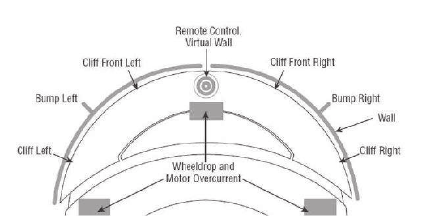
\includegraphics[width=0.7\textwidth]{imagenes/irobot-sensors.png}
	\caption{Ejemplo de sensores en una \textit{Roomba} - Fuente: \textit{ResearchGate} \cite{roomba-sensors-rg}}
\end{figure}

Otro ejemplo mucho más claro de robot lo encontramos en \textbf{\textit{Pepper}} \cite{pepper-robot} (obra de \textit{SoftBank Robotics}), un computador con apariencia \textit{humanoide} con hasta 20 grados de libertad que acepta interacción a través de una pantalla táctil, además de incorporar \textbf{reconomiento vocal} en 15 lenguajes diferentes. Por si fuera poco, a través del \textbf{reconocimiento facial} que hace de los usuarios es capaz de inferir su estado emocional.\\

\begin{figure}[h]
	\centering
	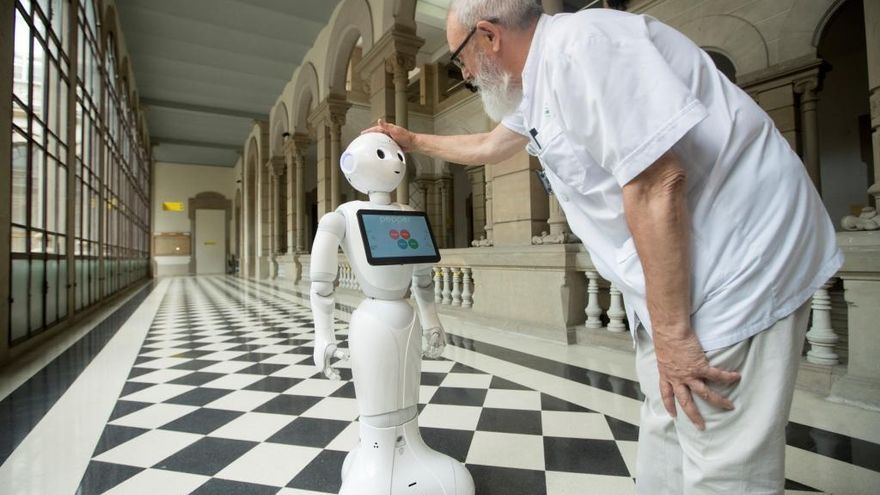
\includegraphics[width=0.7\textwidth]{imagenes/pepper-hospital.jpg}
	\caption{El robot humanoide Pepper proporciona atención a los pacientes en hospitales de Barcelona, brindándoles apoyo moral y entretenimiento - Fuente: \textit{Noticias de Navarra} \cite{pepper-noticias}}
\end{figure}

Si bien el conjunto de avances de inteligencia artifical que realizan los robots de este tipo son espléndidos, no hace falta irse a un plano tan alto para hablar de robótica; ni aunar medidas tan avanzadas de detección y reacción ante el entorno, que también pueden ser usadas por elementos inteligentes que sin embargo no llegan a ser considerados como ``robots''. Podemos encontrar un ejemplo en el \textit{Autopilot}, que es como llama la compañía automovilística de vehículos eléctricos \textit{Tesla} a su sistema de conducción automática \cite{tesla-ai}. Los complejísimos algoritmos de \textbf{visión computacional} que tienen lugar en el vehículo a la hora de observar el entorno en busca de otros coches, peatones, señales y obstáculos; también pasan por un entrenamiento de modelos de inteligencia artificial intenso. La diferencia en el uso de estos, es que (al menos actualmente), aún no existe la conducción plenamente autónoma, y por seguridad aún se requiere que haya un conductor al volante. ¿Podríamos entonces establecer el límite entre lo que es un ``robot'' y lo que no en función de si es necesaria la interacción humana?\\

Responder a ésto es siempre complejo pero interesante, así que me gustaría concluir esa pregunta volviendo al artículo de ``What is a Robot?'' del \textit{IEEE} \cite{whats_a_robot} con la divertida respuesta de \textit{Joseph Engelberger}:

\begin{displayquote}
	``No sé cómo definir un robot, ¡pero sé reconocer uno cuando lo veo!''
\end{displayquote}

\subsubsection{¿Qué necesito para hacer un robot?}

Si quisiéramos crear un nuevo robot, son varios los campos de conocimiento que deberíamos tener en cuenta. Para empezar, la \textbf{electrónica} es algo esencial, ya que su base será la que permitirá controlar el movimiento del dispositivo a través de pulsos de corriente, además de dotarlo de los periféricos de detección y comunicación que hemos mencionado previamente. Por otro lado, el campo de la \textbf{informática} permitirá extender las funcionalidades de este robot dotándole de un sistema operativo y añadiendo aplicaciones sobre la capa abstracta tejida por la electrónica.\\

Si hablamos de hardware, podemos empezar por adquirir una plataforma móvil ya preparada para su uso. Lo primero que puede pensar cualquiera es tomar una como la \textit{Roomba}, cuya movilidad y detección de obstáculos ya está implementada, y sobre ella añadir los componentes y prestaciones que queramos. El problema en cuanto a ésto es que se trata de una \textbf{plataforma cerrada}. No disponer del código fuente hace que no podamos extender el robot como queramos, y así el fabricante se reserva los derechos de su uso.\\

Si no podemos asumir el presupuesto de una plataforma ya montada o simplemente queremos hacer pruebas y divertirnos con la experiencia, hoy en día es fácil y asequible acceder a componentes electrónicos con los que crear pequeños robots y artefactos caseros. Un ejemplo de \textit{núcleo} para ésto sería una placa de \textit{Arduino}, que por unos 20 o 30 euros contiene las conexiones para añadirle módulos de cámara, altavoces, servomotores y cualquier cosa que se nos ocurra \cite{arduino-store}.\\

\begin{figure}[h]
	\centering
	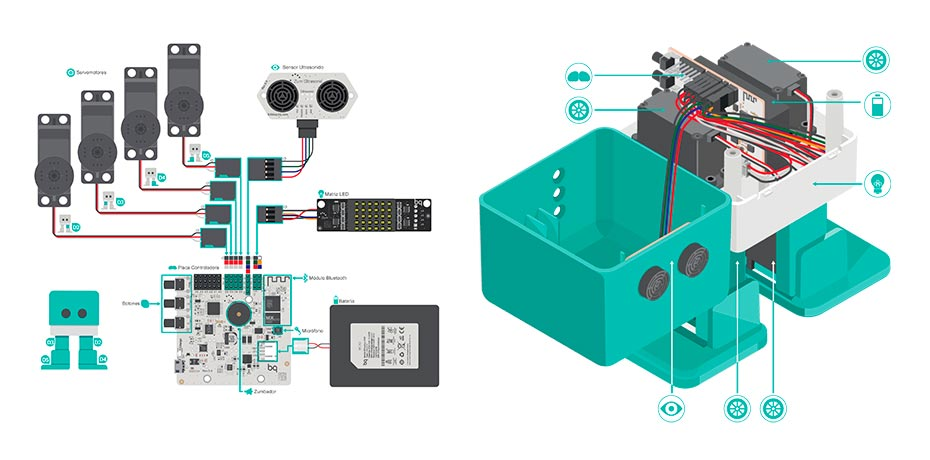
\includegraphics[width=0.9\textwidth]{imagenes/zowi-robot-componentes.jpg}
	\caption{\textit{Zowi}, ejemplo de robot basado en Arduino mas sensores - Fuente: \textit{Balara} \cite{zowi-balara}}
\end{figure}

Esta placa de desarrollo contiene un microcontrolador que permite ser programado en código C muy fácilmente, pero está limitado a eso. Si queremos utilizar un sistema que nos permita gestionar más cosas que la simple ejecución de un código, como un sistema operativo completo, deberíamos dar el salto a algo más parecido a un ordenador común, para lo que puede servirnos la conocida \textit{Raspberry Pi} \cite{raspberry-pi}. Existen otras alternativas de la misma gama provenientes de \textit{Asus} o de \textit{NXP} \cite{nxp-imx}, pero nos ceñiremos a la primera ya que está muy enfocada al sector educativo y al público joven y goza de una comunidad muy numerosa. Lo que todos estos dispositivos comparten son diversas conexiones a través de las cuales podemos añadir los elementos que mencionábamos previamente para nuestro proyecto de robot, además de permitirnos acceso a la configuración de su sistema operativo (o incluso podemos confeccionar uno a nuestra medida, como veremos en el siguiente apartado).\\

\begin{figure}[h]
	\centering
	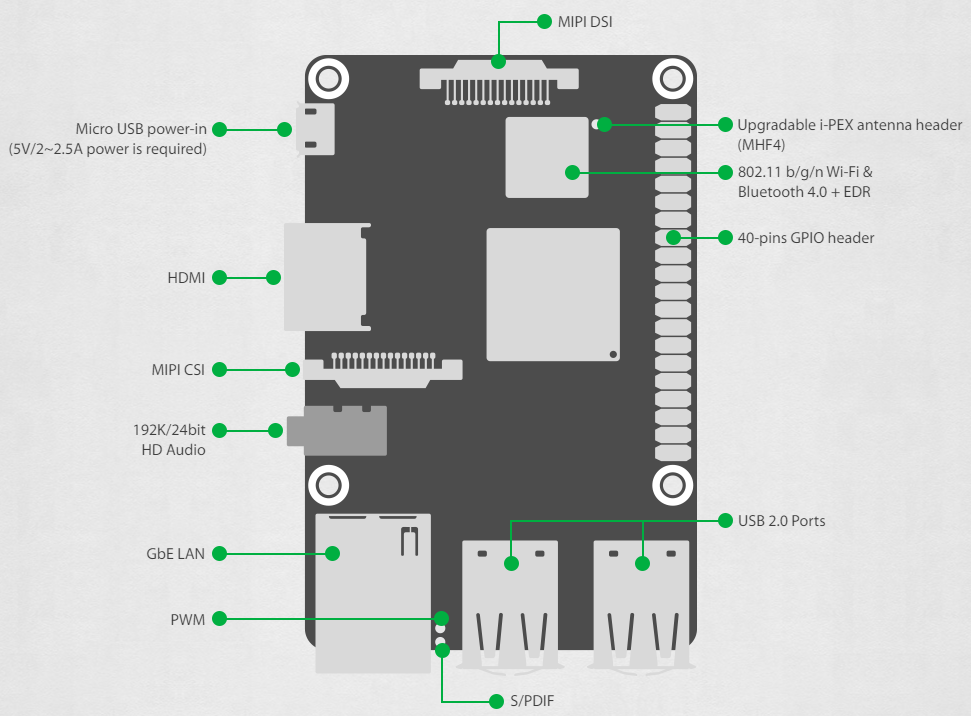
\includegraphics[width=0.75\textwidth]{imagenes/asus-tinker-conexiones.png}
	\caption{\textit{Tinker board}, la alternativa de \textit{Asus} - Fuente: \textit{Asus.com} \cite{asus-tinker}}
\end{figure}


\subsubsection{Sistema operativo, el cerebro del robot}

Continuando con la \textit{Raspberry}, el ordenador monoplaca en torno al cual podríamos construir nuestro robot, pasemos ahora a hablar del sistema operativo. Para esta placa en cuestión existe uno muy aclamado por la gente llamado \textbf{\textit{Raspbian}} \cite{raspbian}, basado en \textit{Debian}, una conocida distribución de \textit{GNU/Linux} que viene de los propios creadores de la \textit{RPi} y dispone de todo lo necesario para formar un sistema de operativo completo, incluyendo hasta interfaz gráfica y aplicaciones de escritorio.\\

Contando con instalar en la tarjeta de memoria un sistema operativo ya montado como éste, podríamos seguir adelante con la conexión de periféricos que conformarán nuestro robot, o quizás nos interese más detenernos un momento a decidir si realmente queremos usar opciones como \textit{Raspbian} o preferimos tener algo personalizado y a nuestra medida.\\

Para los más aventureros, existe la posibilidad de diseñar y compilar un sistema operativo propio (aunque también basado en \textit{GNU/Linux}) con herramientas como \textbf{\textit{Buildroot}} \cite{buildroot} y \textbf{\textit{The Yocto Project}} \cite{yocto-project}. Se tratan de frameworks que permiten compilar una distribución \textit{Linux} a medida según las necesidades del dispositivo embebido en cuestión seleccionando las piezas que lo conforman como si de un puzzle se tratase. Por ejemplo, un robot que no tenga pantalla pero sí informe al usuario mediante efectos sonoros puede prescindir de todos los paquetes gráficos; igual que otro que no necesite conectarse a un router de forma inalámbrica no necesita tener instalados todos los paquetes correspondientes a la gestión de \textit{WiFi}.\\

Por un lado, tenemos la decisión entre utilizar un sistema operativo ya compilado o diseñarlo como hemos comentado. Si miramos el estudio que realizó \textit{Mads Doré Hansen} en su paper \textit{Yocto or Debian for Embedded Systems} \cite{yocto-or-debian} podemos matizar nuestra respuesta en consideración.

\begin{displayquote}
	``\textit{Debian} es bueno para pruebas rápidas y entornos de escritorio con memorias grandes y requisitos bajos de mantenimiento. \textit{Yocto} es bueno para entornos personalizados con soporte a distintas plataformas hardware de poca memoria y que requieren trazabilidad y reusabilidad.
\end{displayquote}

Sobre \textit{Debian}, también menciona que al ser conveniente para pruebas rápidas, muchos equipos de desarrollo comienzan su trabajo en la plataforma embebida utilizándolo, posponiendo tanto el paso a utilizar \textit{Yocto} para diseñar un sistema propio, que terminan postérgandolo infinitamente y no lo realizan nunca. Un argumento a favor de ellos es que la \textbf{curva de aprendizaje} de \textit{Yocto} es grande, dado que requiere compilar todo el sistema para la arquitectura destino, mientras que opciones como \textit{Debian} seguramente ya dispongan de paquetes precompilados.\\

Por ahora, nos conformaremos con saber de la existencia de estas alternativas. Más adelante comentaremos cuál nos resulta más conveniente para el caso que nos ocupa.\\


\subsubsection{Programación del robot}

Pasemos ahora a hablar de \textbf{software}. ¿Qué herramientas necesita un desarrollador para programar su robot? Pues bien, indagando un poco podremos ver que realmente no dista mucho de codificar cualquier otro software convencional.\\

En el artículo de \textit{Codete} citado \cite{codete}, listan por orden de volumen de uso los lenguajes de programación más utilizados para robótica. Podemos ver que todos los lenguajes ahí presentes son de uso general, y que cualquier experiencia que ya podamos tener por ejemplo con \textit{Python} para desarrollo web, nos puede servir para iniciarnos en el mundo de la robótica. Otro ejemplo es \textit{Java}, que si bien también es usado extensamente para aplicaciones de escritorio entre otras, aporta herramientas y librerías que pueden ser muy útiles para recepción y procesamiento de imágenes.\\

Sin embargo, de acuerdo con dicho artículo, el más ampliamente usado es \textit{C} y \textit{C++}, ya que permiten un manejo más eficiente de la memoria y un procesamiento a bajo nivel más cercano al hardware. Además, estos lenguajes colaboran directamente con la API del sistema operativo, utilizando las propias librerías ya presentes en el dispositivo.\\

Por otro lado, cuando se habla de robótica suele salir a colación \textit{\textbf{ROS} (Robot Operating System)} \cite{why-ros}, un proyecto de \textbf{código abierto} que incluye un conjunto de librerías y herramientas con las que no es necesario \textit{reinventar la rueda} para adentrarse en la programación de robótica. En diversos artículos podemos encontrar razones por las que utilizar \textit{ROS} (como en \cite{reasons-ros}):

\begin{itemize}
	\item Se trata de un sistema agnóstico para lenguajes. Permite comunicar un robot programado en \textit{C++} con otro hecho en \textit{Python}, por ejemplo.
	\item Es ligero y de propósito general para cualquier finalidad que tenga el robot en cuestión.
	\item Contiene herramientas de simulación que facilitan el desarrollo del robot antes de requerir el uso físico de electrónica real (lo que puede suponer un ahorro en costes de material).
\end{itemize}

Para un uso modesto, quizá el aspecto más interesante de utilizar \textit{ROS} puede resultar la comunicación entre distintos \textbf{nodos}. Podemos entender como \textit{nodo} cada una de las partes independientes del robot que colabora con el resto. Para un robot hipotético que se desliza sobre el suelo y que mueve los brazos para agarrar cosas, podríamos distinguir entre sus nodos la plataforma móvil, las manos, las cámaras que observan el entorno y un largo etcétera. En cuanto a cómo se comunican estos nodos, podemos plantearlo como un problema de comunicación de distintos servicios cualesquiera. Veamos esto en el siguiente apartado.\\


\subsubsection{¿Cómo se comunican los nodos de un robot?}

Como anticipábamos, podemos entender cada \textbf{nodo} como un servicio independiente que se comunica con el resto a través de algún mecanismo integrado en el sistema operativo.\\

Imaginemos que tenemos un nodo \textbf{principal} que representa el cerebro del robot, y que por tanto es el encargado de ordenar al resto de nodos (\textit{secundarios}) la siguiente acción que deben realizar. Si cada uno de estos elementos es un servicio independiente como hemos dicho, es necesario un método de comunicación para que el principal notifique a los demás mediante un mensaje. Si buscamos métodos de \textbf{comunicación entre procesos}, seguramente el primer resultado que obtengamos sea \textbf{\textit{IPC}}, cuyas siglas (\textit{Inter-Process Communication}) en castellano significan exactamente ``comunicación entre procesos'' \cite{ipc}. En la siguiente figura podemos ver una comparativa de las dos formas de comunicación posibles en este ámbito: \textit{Shared memory} y \textit{Message Passing}\\

\begin{figure}[h]
	\centering
	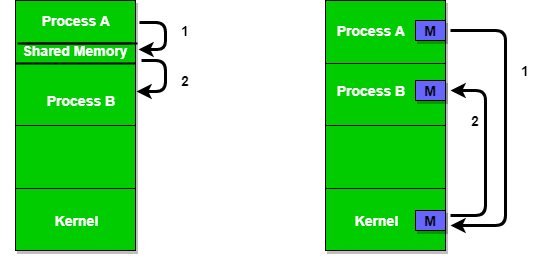
\includegraphics[width=0.7\textwidth]{imagenes/ipc.png}
	\caption{Formas de comunicación \textit{IPC} - Fuente: \textit{GeeksforGeeks.org} \cite{ipc}}
\end{figure}

El método de comunicación mediante \textit{IPC} más inmediato es el uso de \textit{Shared memory} o \textbf{memoria compartida}, que consiste literalmente en reservar un espacio de la memoria lógica para que todos los procesos cooperantes hagan uso de un espacio común donde leer y escribir variables compartidas. Si bien ésto es ágil y rápido, mi experiencia trabajando con esta metodología en proyectos grandes es que si no se tiene especial cuidado a la hora de diseñar qué datos intervienen y su procedencia, a largo plazo ésto produce un gran \textbf{acoplamiento} en el software involucrado.\\

Por otro lado, \textit{Message Passing} (\textbf{paso de mensajes}) consiste en habilitar un búfer compartido a nivel de kernel en el que pueden escribir y leer los procesos interesados. La diferencia con la \textbf{memoria compartida} es que en ésta se pueden utilizar directamente las variables del lenguaje de programación escogido, mientras que con \textbf{paso de mensajes} lo que se hace es escribir objetos completos con un identificador de mensaje. Así, lo que hacen los servicios para leer información es iterar sobre dicho búfer buscando si los identificadores de mensaje presentes son de su interés o no. Con esta aproximación, es sencillo enviar mensajes \textit{1:1} (de un servicio a otro) o \textit{1:n} (\textit{multicast} o \textit{broadcast}) entre servicios concretos.\\

Dejando \textit{IPC} a un lado y volviendo a \textit{ROS}, que antes mencionábamos que es un set de librerías y herramientas bien amplio, destaquemos ahora que también contiene formas de comunicación entre nodos, e incluso su documentación contiene tutoriales sobre cómo empezar a trabajar en ello (como encontramos en \cite{ros-tutorial}, donde enseñan cómo partir con un modelo \textbf{\textit{publicación-suscripción}} en lenguaje \textit{C++}).\\

Este patrón también conocido como \textit{PubSub} se trata de una forma de \textbf{mensajería asíncrona} para integrar microservicios en una arquitectura software. O como detallan en \textit{Amazon AWS} \cite{whats-pubsub}: ``para usar en arquitecturas \textit{serverless} o basadas en \textbf{microservicios}''.\\

El funcionamiento de éste es simple y permite implementar \textbf{arquitecturas basadas en eventos}:

\begin{itemize}
	\item Un \textbf{servicio} se suscribe a un \textbf{tópico}, como lo haría un usuario de la televisión por cable a los canales cuyo contenido le interese.
	\item Otro servicio \textbf{publicará mensajes} en dicho tópico, de forma que el primero los recibirá inmediatamente.
	\item Esta mecánica se generaliza con tantos servicios y tópicos como sea necesario.
\end{itemize}

\begin{figure}[h]
	\centering
	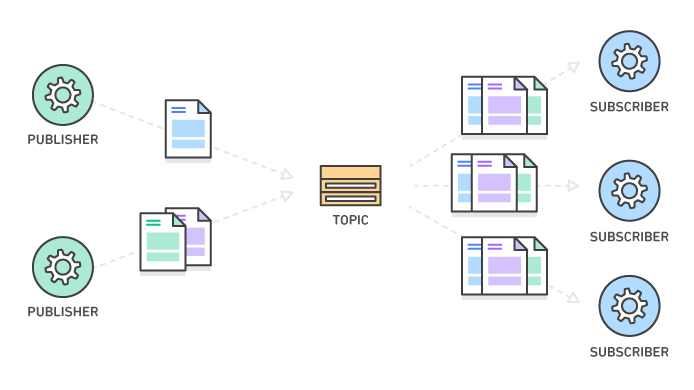
\includegraphics[width=0.7\textwidth]{imagenes/pubsub.png}
	\caption{Mecánica \textit{PubSub}. Dos servicios publican sobre un mismo tópico para que otros tres reciban su contenido inmediatamente - Fuente: \textit{Amazon AWS} \cite{whats-pubsub}}
\end{figure}

Sobre \textit{PubSub}, encontramos también el \textbf{servicio de mensajería \textit{MQTT}}, que funciona de forma similar. En la imagen siguiente. vemos que ahora se sitúan al \textbf{publicador} y al \textbf{suscriptor} a ambos lados de un \textbf{bróker}, que es el responsable de notificar a cada uno de los servicios suscritos cuando se ha añadido un mensaje a su tópico de interés.\\

\begin{figure}[h]
	\centering
	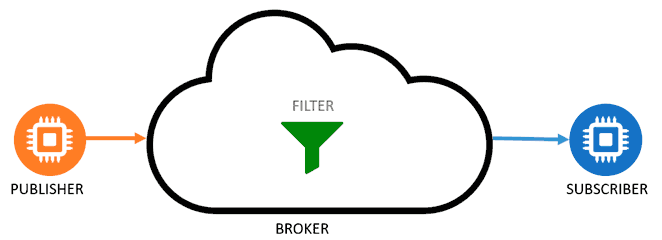
\includegraphics[width=0.6\textwidth]{imagenes/protocolos-iot-pubsub.png}
	\caption{Mensajería \textit{MQTT} con patrón \textbf{publicador/suscriptor}. El bróker intermedio es quien recibe los mensajes que van a cada tópico y notifica a cada servicio suscrito. - Fuente: \textit{Luis Llamas} \cite{mqtt-pubsub}}
\end{figure}

En mi experiencia, el modelo \textit{PubSub} es el más cómodo de utilizar una vez que el proyecto ya está preparado para trabajar en él y añadir funcionalidades, además de gozar de una gran \textbf{escalabilidad}, ya que añadir nuevos mensajes, tópicos y servicios es totalmente transparente y práctico. Bien es cierto que para no reinventar la rueda, es conveniente utilizar librerías que ya implementen este paradigma, como \textit{Redis} o \textit{ROS}, que mencionábamos antes.\\

Si bien hemos visto que \textit{ROS} puede servir para cualquiera que quiera iniciarse en la robótica, \textit{Redis} es una herramienta muy interesante a tener en cuenta para intercomunicar los distintos nodos o procesos que tendrán lugar en el dispositivo. Se trata de un \textbf{almacén de estructuras de datos} que puede actuar como base de datos, caché o bróker de mensajes; que se mantiene en memoria principal, por lo que es volátil a la par que muy rápida \cite{redis}. Además, implementa el paradigma \textit{PubSub}, permitiendo realizar suscripciones a tópicos y/o publicar mensajes sobre ellos. Automáticamente, los programas que utilicen alguna librería de \textit{Redis} son notificados cuando un mensaje es publicado en un tópico al que están suscritos \cite{redis-pubsub}.\\

Dejemos aquí la enumeración y descripción de los distintos módulos software que nos pueden servir para programar el susodicho robot. En apartados posteriores estudiaremos cada una de las decisiones tomadas al respecto.\\


\subsubsection{Conectividad del robot}

Para terminar con el \textit{Estado del Arte}, veamos por último qué opciones hay a la hora de comunicar nuestro robot con la red exterior, en caso de que necesitemos enviar telemetría, recibir órdenes remotas o incluso recabar datos para un servidor.\\

La primera alternativa que nos encontramos se trata del conocido protocolo \textbf{\textit{HTTP}} (\textit{HyperText Transfer Protocol}), que utilizamos a diario cuando consultamos cualquier web a través de nuestro ordenador o teléfono móvil. De acuerdo con la documentación de \textit{Mozilla} \cite{http_protocol}, es un protocolo de escritura cliente-servidor donde la comunicación es iniciada por el \textbf{cliente}, es decir, el interesado en recibir los datos (normalmente una página web). La particularidad de este protocolo es que cada conexión termina en cuanto el servidor provee una respuesta completa al cliente. Veámoslo en la siguiente figura:

\begin{figure}[h]
	\centering
	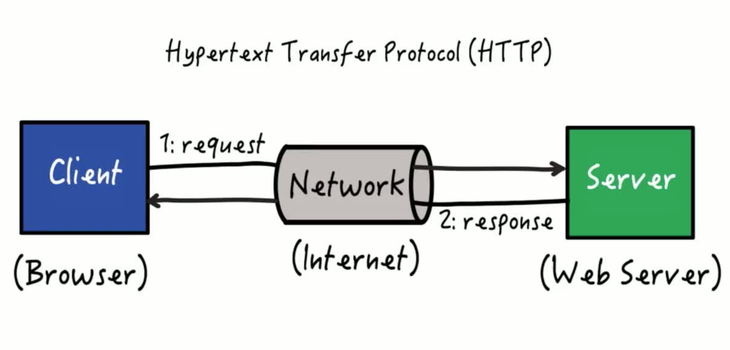
\includegraphics[width=0.7\textwidth]{imagenes/http.png}
	\caption{Funcionamiento del protocolo \textit{HTTP}. Un cliente realiza una petición a través de la red, el servidor recolecta los datos necesarios, los envía al cliente y finaliza la conexión. - Fuente: \textit{Research hubs} \cite{http-image}}
\end{figure}

Una alternativa que encontramos hoy en día al clásico \textit{HTTP} es el protocolo \textbf{\textit{WebSockets}}, que de acuerdo con la documentación para desarrolladores de \textit{Mozilla}: \textit{``es una tecnología que permite abrir una sesión de comunicación \textbf{interactiva} entre el cliente y el servidor''} \cite{ws_protocol}.\\

Las diferencias entre éste y el anterior son:

\begin{itemize}
	\item La conexión en \textit{HTTP} finaliza con cada respuesta exitosa, mientras que en \textit{WebSockets} es interactiva, permaneciendo abierta entre el cliente y el servidor, sin necesidad de reabrirla para cada nueva petición.
	\item \textit{WebSockets} es una tecnología \textbf{basada en eventos}, por lo que no es necesario realizar lecturas periódicas de cara al otro extremo ya que los mensajes enviados por éste \textit{notifican} al servicio que la utiliza.
	\item La comunicación es \textbf{bidireccional}: una vez que se establece la conexión, tanto el cliente como el servidor pueden mandarse mensajes entre sí transparentemente sin necesidad de renegociar el canal de conexión.
\end{itemize}

\begin{figure}[h]
	\centering
	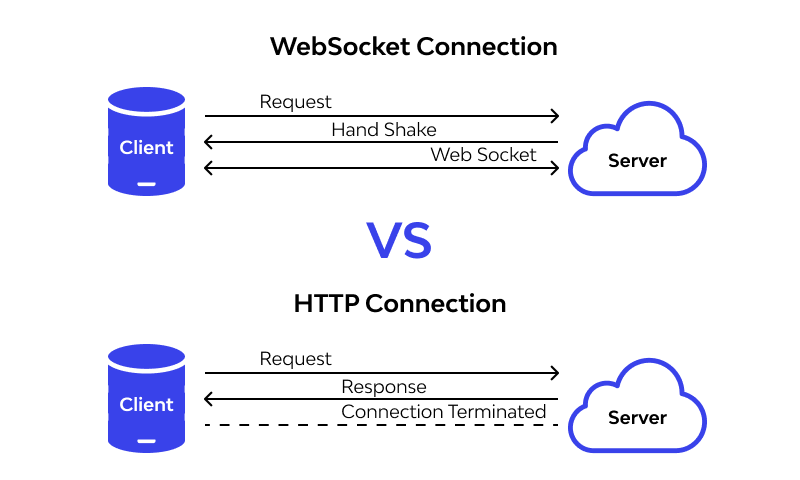
\includegraphics[width=0.8\textwidth]{imagenes/ws_vs_http.png}
	\caption{La diferencia entre la conexión en \textit{WebSocket} y \textit{HTTP} la vemos en la última línea de cada diagrama. En el primer caso el canal permanece abierto y en el segundo se cierra tras la respuesta del servidor. - Fuente: \textit{Wallarm.com} \cite{ws_connection}}
\end{figure}

Para terminar con esta sección, cabe recordar también otra vez \textbf{\textit{MQTT}}, que pese a no ser un protocolo como tal, permitirá orquestar los robots en torno a un servidor de forma que puedan compartir un canal de \textbf{mensajería \textit{push}} sobre un servidor acordado. Este elemento actuaría como \textbf{nodo principal} que podría publicar en distintos tópicos, y los robots actuarían como nodos \textbf{secundarios} y suscritos.\\

Si bien siempre es posible indagar un poco más en todas las alternativas y tecnologías que tenemos disponibles a día de hoy, pasemos de una vez a enumerar los requisitos que regirán el desarrollo de este proyecto.\\















